\documentclass[11pt]{article}
\usepackage[english]{babel}
\usepackage{natbib}
\usepackage{url}
\usepackage[utf8]{inputenc}
\usepackage{amsmath}
\usepackage{amssymb}
\usepackage{graphicx}
\usepackage{parskip}
\usepackage{fancyhdr}
\usepackage{vmargin}
\usepackage{booktabs}
\usepackage[table,xcdraw]{xcolor}
\usepackage{tabularx}
\usepackage{caption} 
\usepackage{float}
\usepackage{longtable}
\usepackage{array}
\usepackage{subcaption}
\usepackage{changepage}


\setmarginsrb{3 cm}{1 cm}{3 cm}{1 cm}{1 cm}{1.5 cm}{1 cm}{1.5 cm}

\newcolumntype{L}[1]{>{\raggedright\let\newline\\\arraybackslash\hspace{0pt}}m{#1}}
\newcolumntype{C}[1]{>{\centering\let\newline\\\arraybackslash\hspace{0pt}}m{#1}}
\newcolumntype{R}[1]{>{\raggedleft\let\newline\\\arraybackslash\hspace{0pt}}m{#1}}

\title{Assignment \#4 - Process Modelling with Neuro-Fuzzy Systems}
\date{\today}

\makeatletter
\let\thetitle\@title
\let\thesubtitle\@subtitle
\let\theauthor\@author
\let\thedate\@date
\makeatother

\pagestyle{plain}

\captionsetup[table]{skip=5pt}


\begin{document}

%%%%%%%%%%%%%%%%%%%%%%%%%%%%%%%%%%%%%%%%%%%%%%%%%%%%%%%%%%%%%%%%%%%%%%%%%%%%%%%%%%%%%%%%%

\begin{titlepage}
	\centering
    \textsc{\LARGE University of Coimbra}\\[1.0 cm]
	\textsc{\large Doctoral Program in Information Science and Technology}\\[0.5 cm]
    \textsc{\large Real Time Learning in Intelligent Systems}\\[5 cm]
	\rule{\linewidth}{0.2 mm} \\[0.4 cm]
	{ \LARGE \bfseries \thetitle}\\ [0.2 cm]
    \rule{\linewidth}{0.2 mm} \\[3 cm]
    
    \textsc{Joaquim Pedro Bento Gonçalves Pratas Leitão - 2011150072}\\[5 cm]
	
	{\large \thedate}\\[2 cm]
 
	\vfill
	
\end{titlepage}

%%%%%%%%%%%%%%%%%%%%%%%%%%%%%%%%%%%%%%%%%%%%%%%%%%%%%%%%%%%%%%%%%%%%%%%%%%%%%%%%%%%%%%%%%

\section{Introduction}
\label{introduction}

Dynamic systems are often described and modelled by difference equations, where the outputs in a given time instant (say k) are conditioned by previous outputs (in instants $k-1$, $k-2$, ...) and inputs (in instants $k$, $k-1$, $k-2$, ...). A system is also said to have \emph{inertia} when the inputs in a given instant only affect its outputs in posterior instants (that is, input at instant $k$ can only influence the output at instants $k+1$, $k+2$, ...).

The current assignment proposes the development of a Sugeno-type Neuro-Fuzzy System (NFS) to model the dynamics of a given process or system with inertia. NFSs of this nature are characterised by mapping their input space to an output space using a series of fuzzy \emph{if-then} rules. In the particular case of Sugeno NFSs the output of each rule is written as a linear combination of the input variables. In simpler Sugeno systems, this linear combination consists in a constant value.

By collecting data containing pairs of the system's input and corresponding output values the rules that define the NFS can be learned in such a way that they describe the system's behaviour.

In other words, exploring collected data from the system the mentioned fuzzy rules can be learned, resulting in the development of a Sugeno NFS that models the dynamics of the desired process or system, as it is the objective of this assignment.

The remainder of this document is organised as follows: Section \ref{modelled_system} presents the system to be modelled in this work; Section \ref{methodology} describes the methodology followed throughout the project; Sections \ref{fase_a} and \ref{fase_b} cover the main steps of the work, presented in the Methodology section. Finally, Section \ref{conclusion} concludes the document.


\section{Modelled System}
\label{modelled_system}

The system to be modelled in this work can be defined by the following transfer function:

$$ G(s) = \frac{2}{s^{3} + 5s^{2} + 6.75s + 2.25}$$

Since the provided transfer function features $3$ poles and no zeros - therefore it has more poles than zeros - the presented system is a third-order system. It can be proved that the provided system has memory of $3$ instants in both the inputs and outputs and \emph{inertia} (meaning that inputs at a given time instant only influence future outputs). In this sense, the output of the system at any time instant $k$ can be written as:

$$ y(k) = f(y(k-1), y(k-2), y(k-3), u(k-1), u(k-2),u(k-3))$$

where $y(k)$ represents the system's output at instant $k$ and $u(k)$ represents the system's input at instant $k$.

\section{Methodology}
\label{methodology}

The project and development of a Neuro-Fuzzy System can be a complex and extensive task. Nevertheless, in the scope of the current work, the following two main steps will be considered:

\begin{enumerate}
	\item \textsc{Learning Stage}, where a model of the system is learned using data collected from the system. This stage comprises three main sub-tasks:
	
	\begin{itemize}
		\item \emph{Data collection}, where pairs of system's \emph{input-output} data are collected, which will be used as a labelled dataset during the learning. Collecting a good set of \emph{input-output} data is critical in the final outcome. These data should be representative of the dynamics of the system, making the input and output vary over the entire permissible domain. A good technique is to use a random input sequence that forces the output to move through the entire space.
		
		\item \emph{Fuzzy rules initialisation}. An initial estimate for the NFS's rules is obtained by applying a \emph{clustering} algorithm to the labelled dataset collected in the previous point. Common algorithms used at this stage include subtractive, c-means and fuzzy c-means clustering.
		
		\item \emph{Fuzzy rules optimisation}. A further optimisation of the fuzzy rules computed in the previous point is usually performed, aiming to reduce the modelling error. An \emph{ANFIS} structure is commonly used along with either a \emph{backpropagation} or \emph{hybrid} optimisation method (although other alternatives maybe considered at this point).
		
	\end{itemize}
	
	\item \textsc{Assessment Stage}, where different input signals are provided to both the developed model and the real system with the objective of comparing the real and simulated outputs. The ultimate goal of this task is to certify that the developed model of the system can accurately describe its behaviour.
\end{enumerate}

\section{Learning Stage}
\label{fase_a}

As presented in the previous section, the goal of the \emph{Learning Stage} is to train a Neuro-Fuzzy System to model the target system's behaviour based on pairs of \emph{input-output} signals collected from the target system.

Therefore the first step of this stage is related with data collection. Since no access to the \emph{"real", physical} system is available data will be collected with \emph{Simulink}, a graphical programming and simulation environment available with the \emph{MATLAB} software.

\subsection{Data Collection}
\label{data_collection}

Usually, the process of collecting data from a given system assumes that the collection is made at a given frequency, meaning that samples are collected with a given interval. It is recommended that the sampling interval (also referred to as discretization interval) be less than the inverse of the smaller pole of the system. As such, a sampling interval equal to one-third of the inverse of the smaller pole of the system was used.

After setting the sampling interval, a discrete version of the system's transfer function must be computed. Resorting to the \emph{MATLAB} software environment, such computation can be performed with the function \emph{c2dm}. The following discrete transfer function was obtained:

$$ G(z) = \frac{0.1079z^{2} + 0.1413z + 0.009003}{z^{3} - 0.8794z^{2} + 0.1766z - 0.006738}$$

In this sense, the block diagram presented in Figure \ref{input_generator_block_diagram} was created. A random number generator is used to produce random inputs to the system to which the corresponding outputs are obtained. Both the generated inputs and outputs are stored in memory. The system dynamics are simulated during a total simulation time of $500$ instants. The generated data was further divided into a \emph{training} and \emph{testing} dataset, with a $70-30$ division.

\begin{figure}[ht]
	\centering
	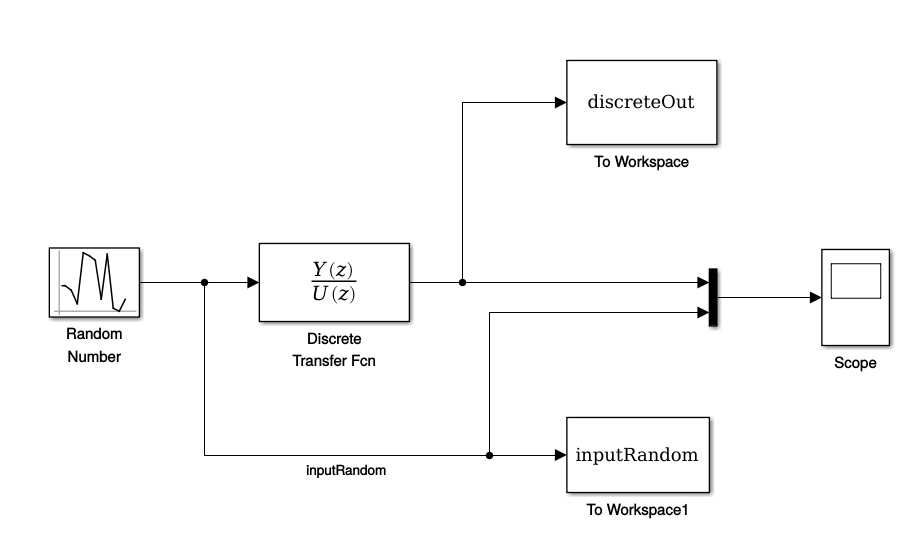
\includegraphics[scale=0.4]{images/input_generator_block_diagram.png}
	\caption{Block diagram developed in Simulink to generate training and testing data.}
	\label{input_generator_block_diagram}
\end{figure}

The generated input signal and correspondent system's output is presented in Figure \ref{generated_input_output}:

\begin{figure}[ht]
	\centering
	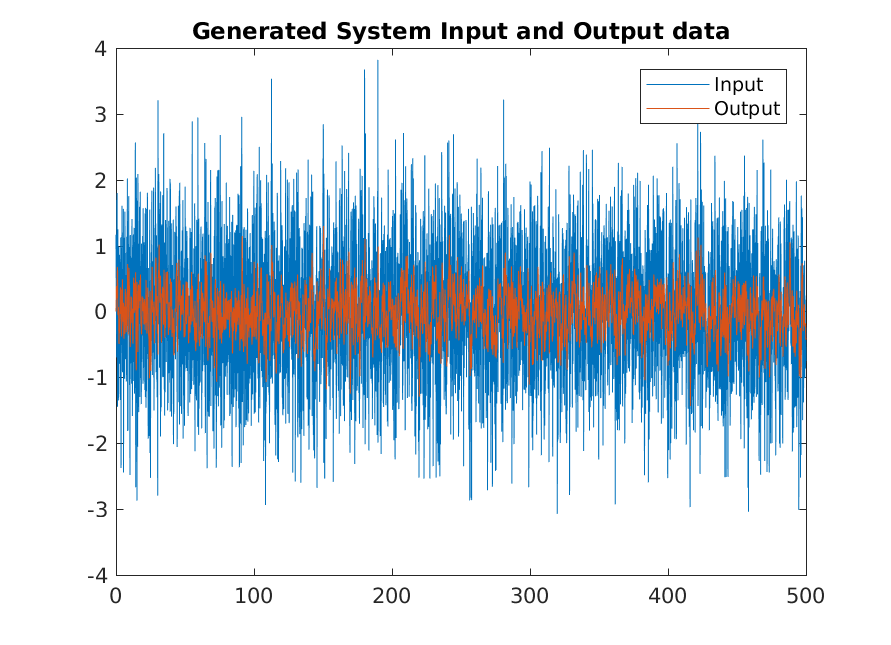
\includegraphics[scale=0.5]{images/randomInputOutput.png}
	\caption{Generated input signal and system output.}
	\label{generated_input_output}
\end{figure}


\subsection{Fuzzy Rules Initialisation}

Having generated input and output samples representative of the dynamics of the system being modelled, the actual learning process can be started. As mentioned in Section \ref{methodology}, in an initial step, estimations for the fuzzy rules are produced as a result of a clustering process of the collected data. Two clustering algorithms were studied at this point, featuring the following parameters:

\begin{itemize}
	\item \textsc{Subtractive Clustering}, where a \emph{cluster influence range} of $0.5$ was defined; s \emph{squash factor} of $1.25$ was considered, along with an accept ratio of $0.5$ and reject ratio of $0.15$.
	
	\item \textsc{Fuzzy C-Means Clustering}, considering an exponent for the fuzzy partition matrix of $2.0$, maximum number of iterations of $100$, minimum improvement in objective function between two consecutive iterations of $10^{-5}$ and the number of clusters being automatically estimated using subtractive clustering.
\end{itemize}

In terms of implementation, the initial estimation of the fuzzy rules was performed using the \emph{MATLAB's genfis} function, properly specifying the training data, the type of clustering to be performed and the respective parameters. The last two arguments (type of clustering and clustering parameters) were defined by creating a proper \emph{genfisOptions} object.

The remainder of the current subsection presents a detailed view of the fuzzy inference systems obtained after the initial rules estimation.

\begin{table}[ht]
	\centering
	\caption{Fuzzy Inference Systems obtained after the initial rules estimation.}
	\begin{tabular}{|c|c|c|c|c|}
		\hline
		\textbf{Cluster Technique} & \textbf{AND Method} & \textbf{OR Method} & \textbf{Order} \\ \hline
		Subtractive & Product & \begin{tabular}[c]{@{}c@{}}Probabilistic OR of\\ fuzzified input values\end{tabular} & 1 \\ \hline
		Fuzzy C-Means & Product & \begin{tabular}[c]{@{}c@{}}Probabilistic OR of\\ fuzzified input values\end{tabular} & 1 \\ \hline
	\end{tabular}
\end{table}

% ============= Subtractive Clustering

\begin{table}[ht]
	\centering
	\caption{Input Membership Functions - Subtractive Clustering.}
	\begin{tabular}{|c|c|c|}
		\hline
		\textbf{Input Number} & \textbf{Membership Function Type} & \textbf{Parameters} \\ \hline
		in1 & Gaussian Curve (gaussmf) & \begin{tabular}[c]{@{}c@{}}$\sigma = [0.1095; 0.1095; 0.1095]$ \\ $C = [-0.0221; 0.1294; -0.1326]$ \end{tabular} \\ \hline
		in2 & Gaussian Curve (gaussmf) & \begin{tabular}[c]{@{}c@{}}$\sigma = [0.1095; 0.1095; 0.1095]$ \\ $C = [-0.0242; 0.1236; -0.1426]$ \end{tabular} \\ \hline
		in3 & Gaussian Curve (gaussmf) & \begin{tabular}[c]{@{}c@{}}$\sigma = [0.1095; 0.1095; 0.1095]$ \\ $C = [-0.0276; 0.1155; -0.1513]$ \end{tabular} \\ \hline
		in4 & Gaussian Curve (gaussmf) & \begin{tabular}[c]{@{}c@{}}$\sigma = [1.2188; 1.2188; 1.2188]$ \\ $C = [-0.056; -0.0963; 0.2091]$ \end{tabular} \\ \hline
		in5 & Gaussian Curve (gaussmf) & \begin{tabular}[c]{@{}c@{}}$\sigma = [1.2188; 1.2188; 1.2188]$ \\ $C = [0.1841; -0.2404; -0.0825]$ \end{tabular} \\ \hline
		in6 & Gaussian Curve (gaussmf) & \begin{tabular}[c]{@{}c@{}}$\sigma = [1.2188; 1.2188; 1.2188]$ \\ $C = [0.0674; -0.021; -0.0921]$ \end{tabular} \\ \hline
	\end{tabular}
\end{table}

\pagebreak

\begin{figure}[ht]
	\centering
	\begin{subfigure}[t]{0.3\textwidth}
		\centering
		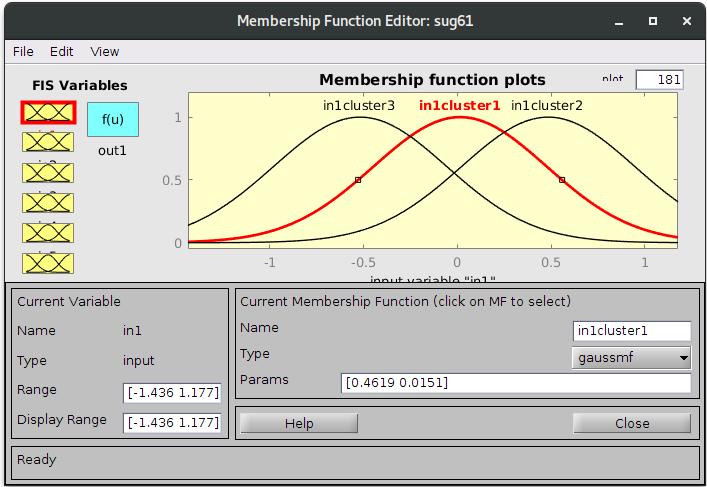
\includegraphics[height=1.2in]{images/subtractive_in1}
		\caption{Membership Functions for input $in1$}
	\end{subfigure}
	~ 
	\begin{subfigure}[t]{0.3\textwidth}
		\centering
		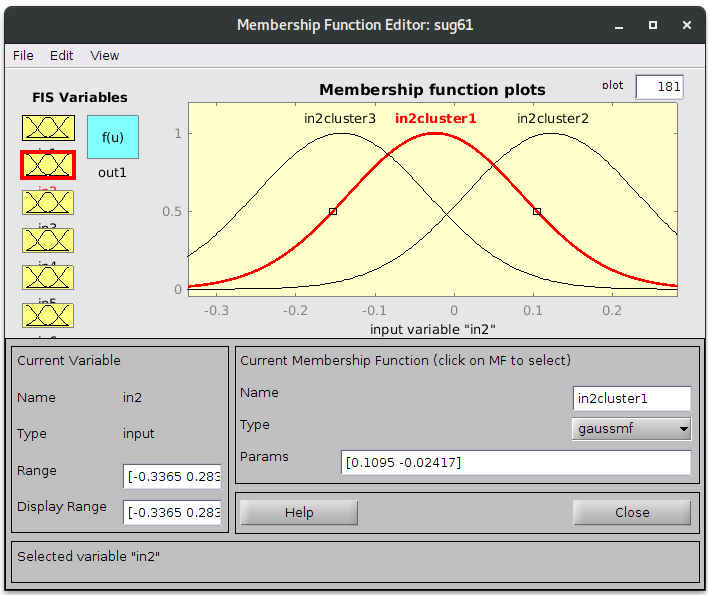
\includegraphics[height=1.2in]{images/subtractive_in2}
		\caption{Membership Functions for input $in2$}
	\end{subfigure}
	~
	\begin{subfigure}[t]{0.3\textwidth}
		\centering
		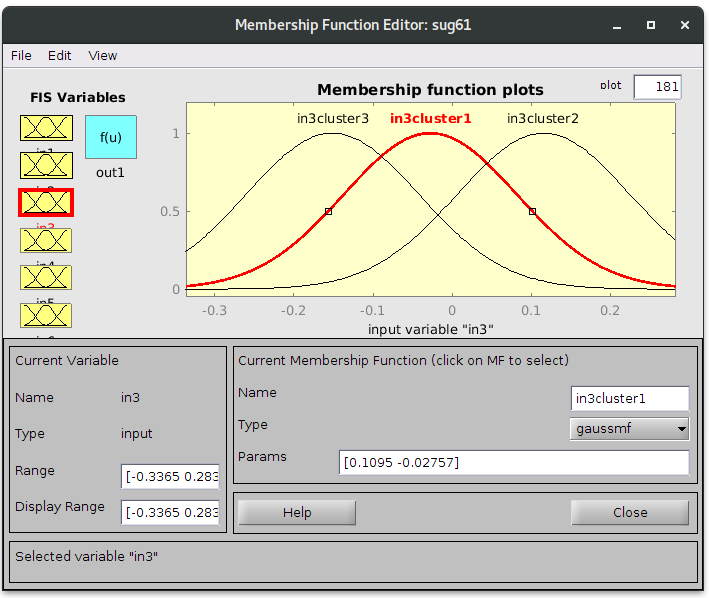
\includegraphics[height=1.2in]{images/subtractive_in3}
		\caption{Membership Functions for input $in3$}
	\end{subfigure}
	\\
	\begin{subfigure}[t]{0.3\textwidth}
		\centering
		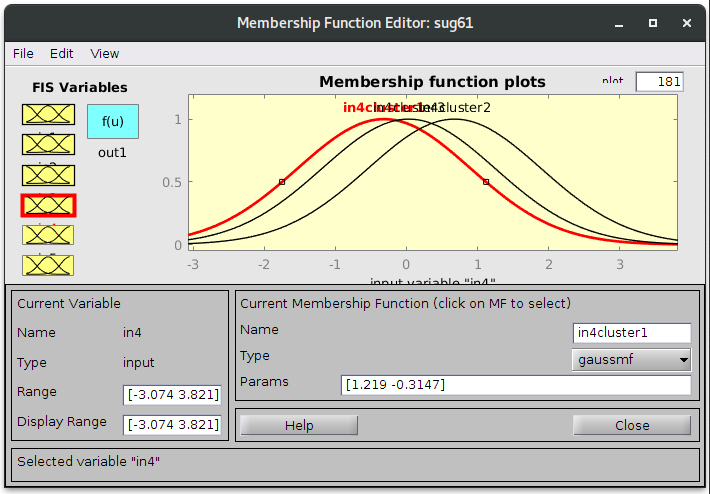
\includegraphics[height=1.2in]{images/subtractive_in4}
		\caption{Membership Functions for input $in4$}
	\end{subfigure}
	~ 
	\begin{subfigure}[t]{0.3\textwidth}
		\centering
		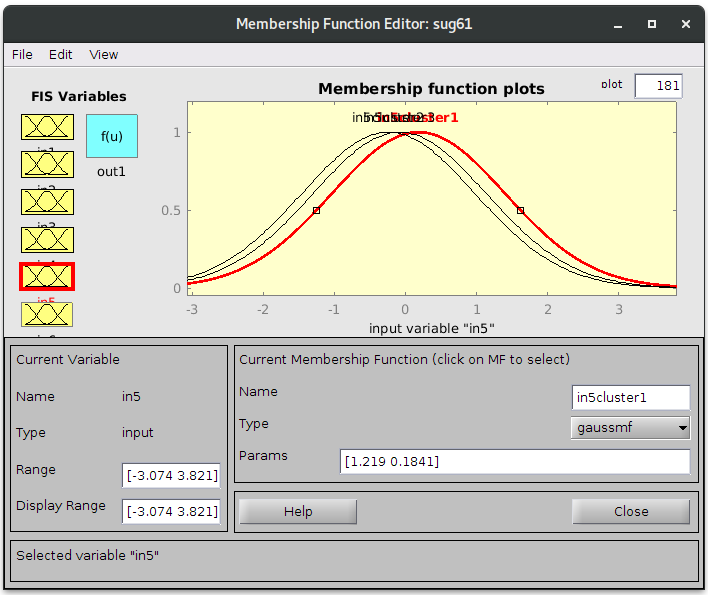
\includegraphics[height=1.2in]{images/subtractive_in5}
		\caption{Membership Functions for input $in5$}
	\end{subfigure}
	~
	\begin{subfigure}[t]{0.3\textwidth}
		\centering
		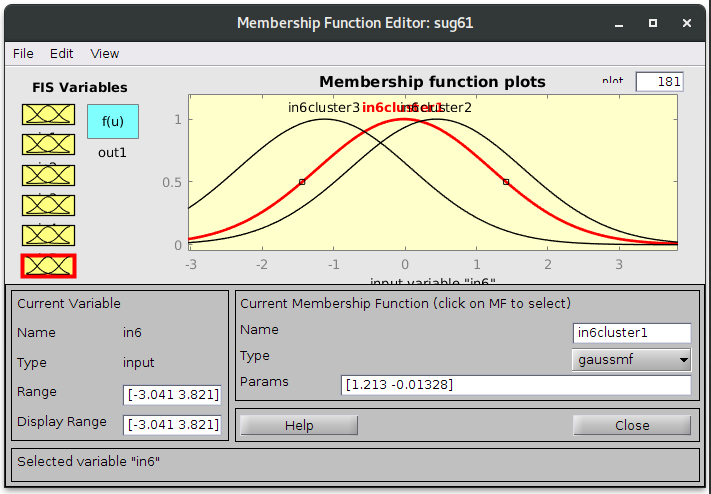
\includegraphics[height=1.2in]{images/subtractive_in6}
		\caption{Membership Functions for input $in6$}
	\end{subfigure}
	\caption{Input Membership Functions for the initial rules obtained with the Subtractive Clustering method.}
\end{figure}

% ============= Fuzzy C-Means Clustering

\begin{table}[ht]
	\centering
	\caption{Input Membership Functions - Fuzzy C-Means Clustering.}
	\begin{tabular}{|c|c|c|}
		\hline
		\textbf{Input Number} & \textbf{Membership Function Type} & \textbf{Parameters} \\ \hline
		in1 & Gaussian Curve (gaussmf) & \begin{tabular}[c]{@{}c@{}}$\sigma = [0.0636; 0.0638; 0.0636]$ \\ $C = [-0.0086; -0.0071; -0.0108]$ \end{tabular} \\ \hline
		in2 & Gaussian Curve (gaussmf) & \begin{tabular}[c]{@{}c@{}}$\sigma = [0.0637; 0.0637; 0.0636]$ \\ $C = [-0.0098; -0.0069; -0.0099]$ \end{tabular} \\ \hline
		in3 & Gaussian Curve (gaussmf) & \begin{tabular}[c]{@{}c@{}}$\sigma = [0.0637; 0.0637; 0.0635]$ \\ $C = [-0.0101; -0.0069; -0.0097]$ \end{tabular} \\ \hline
		in4 & Gaussian Curve (gaussmf) & \begin{tabular}[c]{@{}c@{}}$\sigma = [0.5497; 0.5851; 0.5863]$ \\ $C = [-0.0334; -0.4924; 0.4953]$ \end{tabular} \\ \hline
		in5 & Gaussian Curve (gaussmf) & \begin{tabular}[c]{@{}c@{}}$\sigma = [0.5592; 0.5909; 0.5669]$ \\ $C = [-0.2425; 0.5136; -0.3109]$ \end{tabular} \\ \hline
		in6 & Gaussian Curve (gaussmf) & \begin{tabular}[c]{@{}c@{}}$\sigma = [0.6152; 0.5591; 0.5746]$ \\ $C = [0.6764; -0.2763; -0.4373]$ \end{tabular} \\ \hline
	\end{tabular}
\end{table}

\pagebreak

\begin{figure}[ht]
	\centering
	\begin{subfigure}[t]{0.3\textwidth}
		\centering
		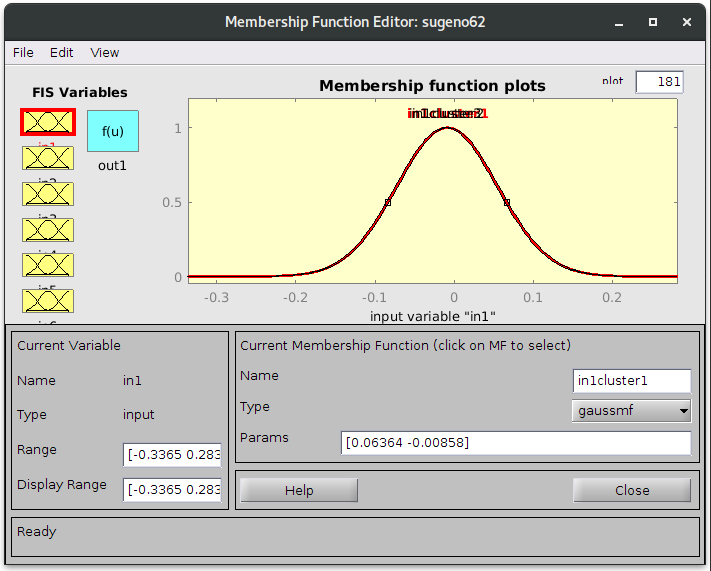
\includegraphics[height=1.2in]{images/fcm_in1}
		\caption{Membership Functions for input $in1$}
	\end{subfigure}
	~ 
	\begin{subfigure}[t]{0.3\textwidth}
		\centering
		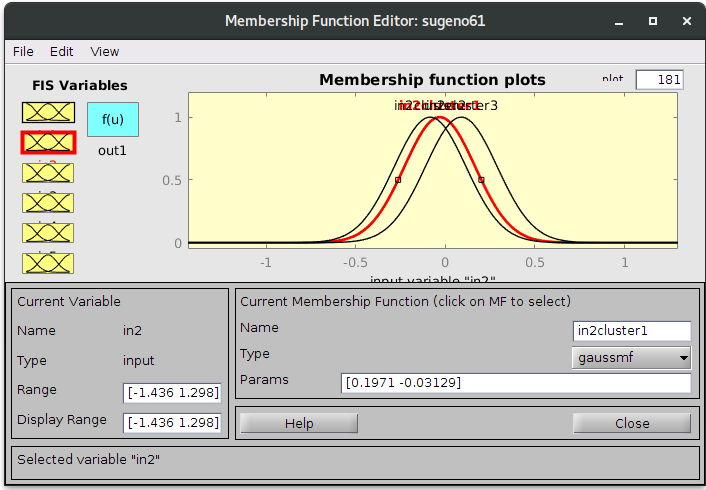
\includegraphics[height=1.2in]{images/fcm_in2}
		\caption{Membership Functions for input $in2$}
	\end{subfigure}
	~
	\begin{subfigure}[t]{0.3\textwidth}
		\centering
		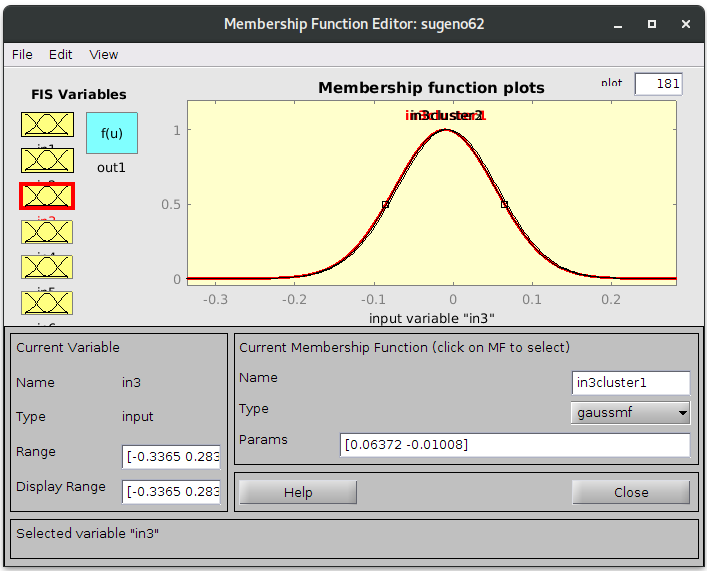
\includegraphics[height=1.2in]{images/fcm_in3}
		\caption{Membership Functions for input $in3$}
	\end{subfigure}
	\\
	\begin{subfigure}[t]{0.3\textwidth}
		\centering
		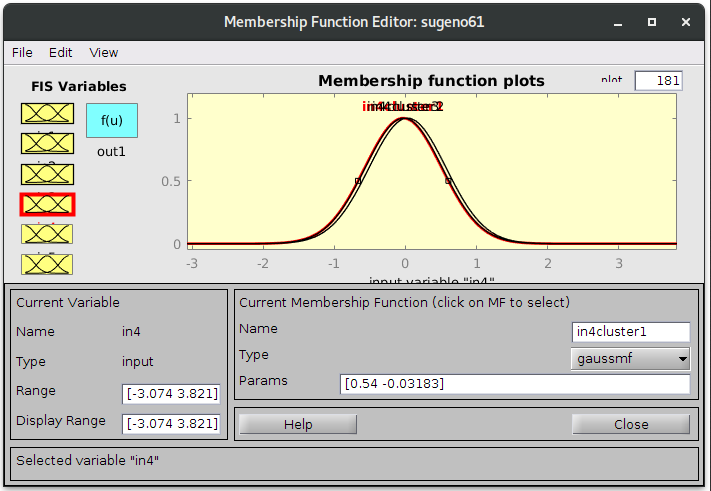
\includegraphics[height=1.2in]{images/fcm_in4}
		\caption{Membership Functions for input $in4$}
	\end{subfigure}
	~ 
	\begin{subfigure}[t]{0.3\textwidth}
		\centering
		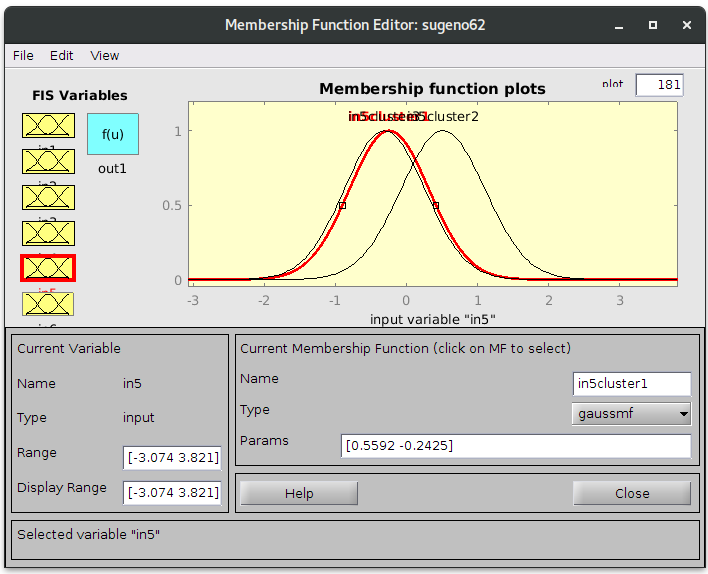
\includegraphics[height=1.2in]{images/fcm_in5}
		\caption{Membership Functions for input $in5$}
	\end{subfigure}
	~
	\begin{subfigure}[t]{0.3\textwidth}
		\centering
		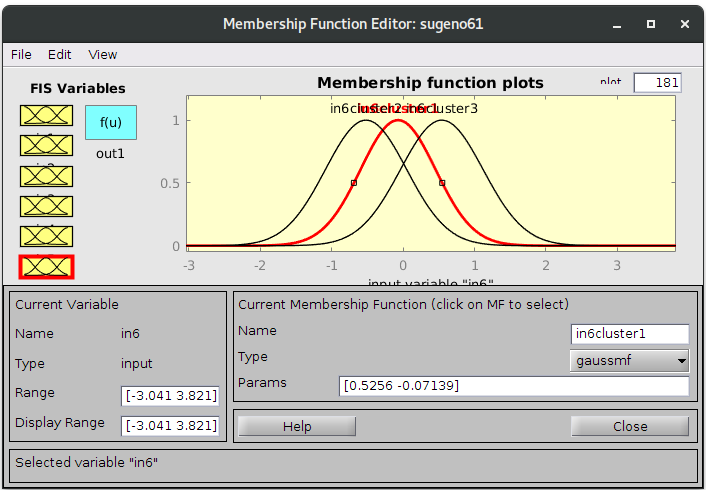
\includegraphics[height=1.2in]{images/fcm_in6}
		\caption{Membership Functions for input $in6$}
	\end{subfigure}
	\caption{Input Membership Functions for the initial rules obtained with the Fuzzy C-Means Clustering method.}
\end{figure}

\subsection{Fuzzy Rules Optimisation}

In the final step of the learning stage an ANFIS structure is used to optimise the estimations for the fuzzy rules obtained in the previous subsection. Two optimisation methods were considered at this point: the well-known \emph{Backpropagation} and an \emph{Hybrid} method.

In terms of implementation, the optimisation of the inference rules was performed using \emph{MATLAB}'s \emph{anfis} function, properly specifying the training data, the type of optimisation method and the number of epochs\footnote{A value of $200$ was defined for the epoch number.}. The last two arguments (type of optimisation and the number of epochs) were defined by creating a proper \emph{anfisOptions} object.

Analysing the input membership functions of the optimised Neuro-Fuzzy Systems (NFS) no changes were registered in the NFSs where the backpropagation optimisation method was used; however, visible changes in the mean and deviation of the gaussians were registered when the hybrid optimisation method was used along with both fuzzy c-means and subtractive clustering. Tables \ref{final_results_hybrid_subtractive}  and \ref{final_results_hybrid_fcm} presents the new input membership functions.

\pagebreak

\begin{table}[ht]
	\centering
	\caption{Final Input Membership Functions - Subtractive Clustering and Hybrid Optimisation Method.}
	\label{final_results_hybrid_subtractive}
	\begin{tabular}{|c|c|c|}
		\hline
		\textbf{Input Number} & \textbf{Membership Function Type} & \textbf{Parameters} \\ \hline
		in1 & Gaussian Curve (gaussmf) & \begin{tabular}[c]{@{}c@{}}$\sigma = [0.2036; 6.5753e-05; 0.0723]$ \\ $C = [-0.0207; 0.2147; -0.1315]$ \end{tabular} \\ \hline
		in2 & Gaussian Curve (gaussmf) & \begin{tabular}[c]{@{}c@{}}$\sigma = [0.2036; 0.0641; 0.0702]$ \\ $C = [-0.0219; 0.1512; -0.1613]$ \end{tabular} \\ \hline
		in3 & Gaussian Curve (gaussmf) & \begin{tabular}[c]{@{}c@{}}$\sigma = [0.2032; 0.0692; -2.2305e-05]$ \\ $C = [-0.0237; 0.1266; -0.2394]$ \end{tabular} \\ \hline
		in4 & Gaussian Curve (gaussmf) & \begin{tabular}[c]{@{}c@{}}$\sigma = [1.2305; 1.2134; 1.2130]$ \\ $C = [-0.0553; -0.0965; 0.2101]$ \end{tabular} \\ \hline
		in5 & Gaussian Curve (gaussmf) & \begin{tabular}[c]{@{}c@{}}$\sigma = [1.2313; 1.2134; 1.2135]$ \\ $C = [0.1815; -0.2415; -0.0827]$ \end{tabular} \\ \hline
		in6 & Gaussian Curve (gaussmf) & \begin{tabular}[c]{@{}c@{}}$\sigma = [1.2294; 1.2135; 1.2138]$ \\ $C = [0.0644; -0.0212; -0.0924]$ \end{tabular} \\ \hline
	\end{tabular}
\end{table}

\begin{figure}[ht]
	\centering
	\begin{subfigure}[t]{0.3\textwidth}
		\centering
		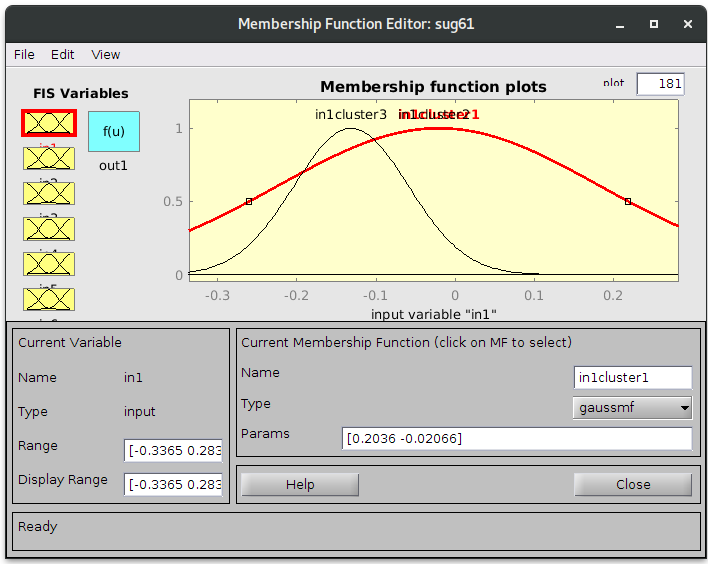
\includegraphics[height=1.2in]{images/subtractive_hybrid_in1}
		\caption{Membership Functions for input $in1$}
	\end{subfigure}
	~ 
	\begin{subfigure}[t]{0.3\textwidth}
		\centering
		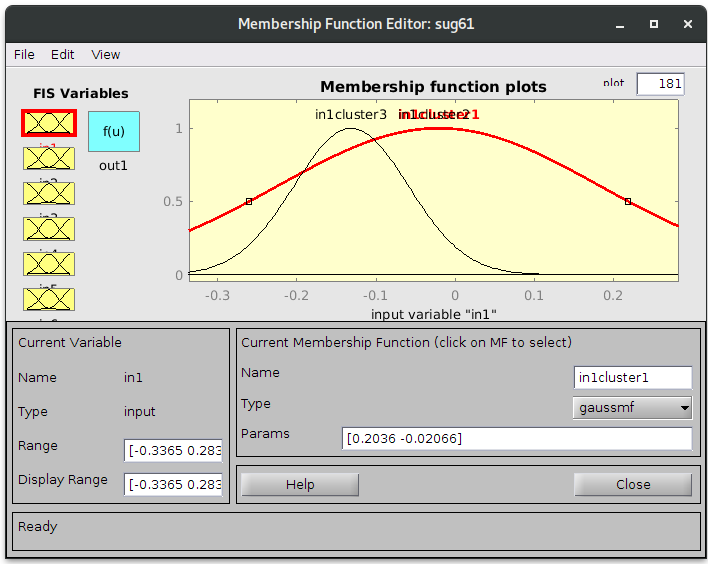
\includegraphics[height=1.2in]{images/subtractive_hybrid_in1}
		\caption{Membership Functions for input $in2$}
	\end{subfigure}
	~
	\begin{subfigure}[t]{0.3\textwidth}
		\centering
		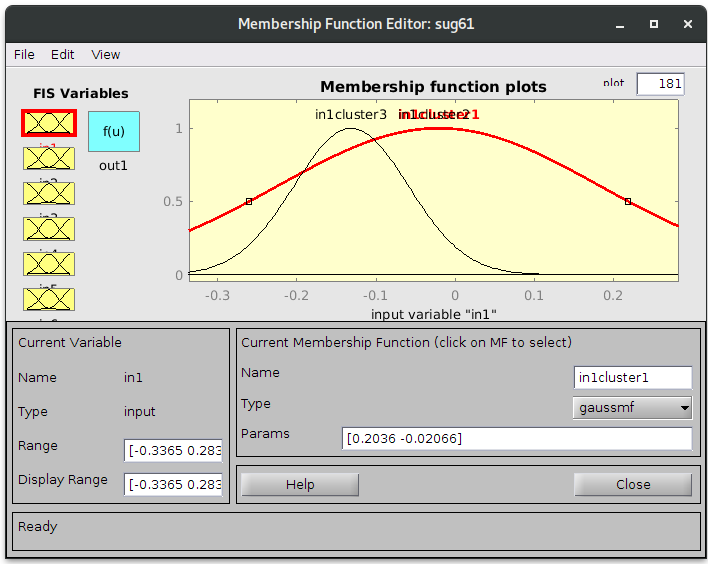
\includegraphics[height=1.2in]{images/subtractive_hybrid_in1}
		\caption{Membership Functions for input $in3$}
	\end{subfigure}
	\\
	\begin{subfigure}[t]{0.3\textwidth}
		\centering
		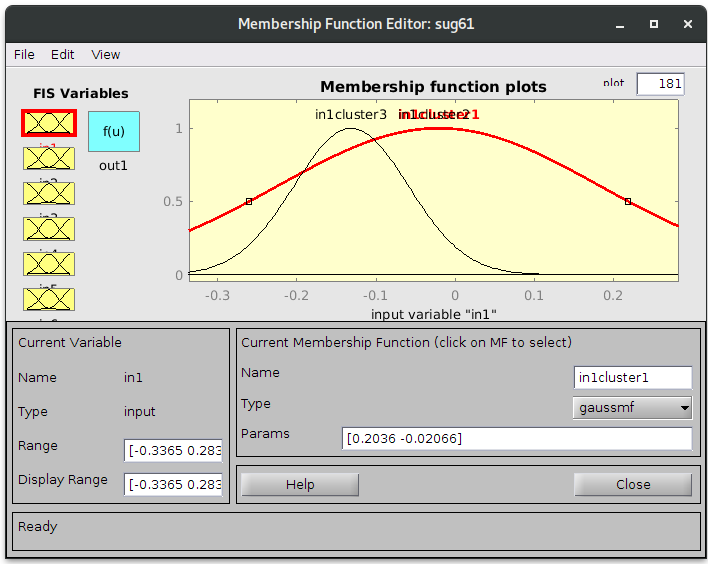
\includegraphics[height=1.2in]{images/subtractive_hybrid_in1}
		\caption{Membership Functions for input $in4$}
	\end{subfigure}
	~ 
	\begin{subfigure}[t]{0.3\textwidth}
		\centering
		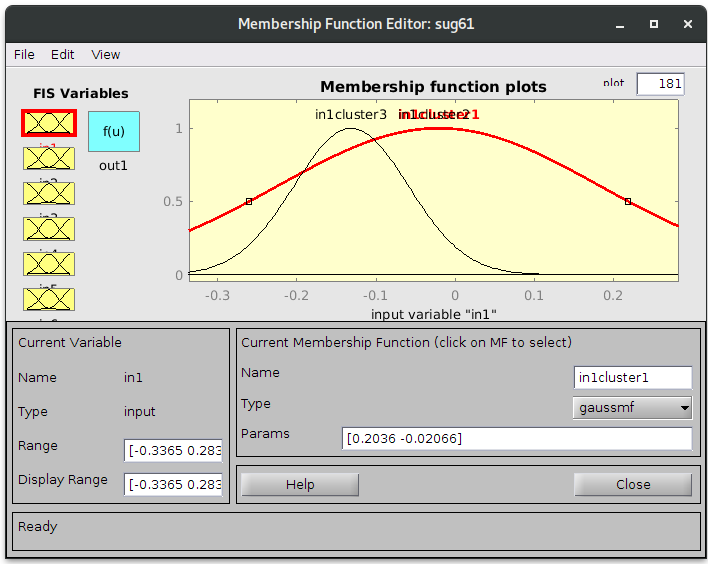
\includegraphics[height=1.2in]{images/subtractive_hybrid_in1}
		\caption{Membership Functions for input $in5$}
	\end{subfigure}
	~
	\begin{subfigure}[t]{0.3\textwidth}
		\centering
		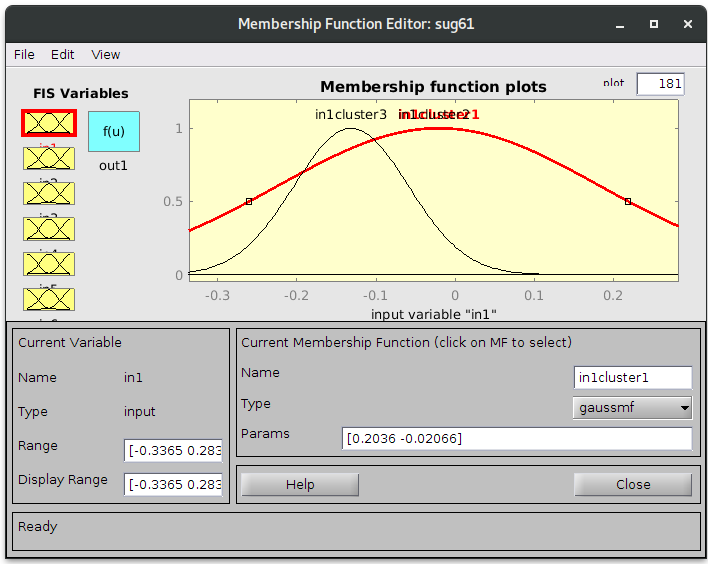
\includegraphics[height=1.2in]{images/subtractive_hybrid_in1}
		\caption{Membership Functions for input $in6$}
	\end{subfigure}
	\caption{Input Membership Functions after Hybrid optimisation when Subtractive Clustering method was used in the rules initialisation.}
\end{figure}

\pagebreak

\begin{table}[ht]
	\centering
	\caption{Final Input Membership Functions - Fuzzy C-Means Clustering and Hybrid Optimisation Method.}
	\label{final_results_hybrid_fcm}
		\begin{tabular}{|c|c|c|}
		\hline
		\textbf{Input Number} & \textbf{Membership Function Type} & \textbf{Parameters} \\ \hline
		in1 & Gaussian Curve (gaussmf) & \begin{tabular}[c]{@{}c@{}}$\sigma = [-2.3364e-04; 0.0964; -0.0021]$ \\ $C = [-0.0305; -0.0128; 0.0204]$ \end{tabular} \\ \hline
		in2 & Gaussian Curve (gaussmf) & \begin{tabular}[c]{@{}c@{}}$\sigma = [0.0145; 0.0966; 2.1969e-04]$ \\ $C = [-0.0058; -0.0133; -0.0145]$ \end{tabular} \\ \hline
		in3 & Gaussian Curve (gaussmf) & \begin{tabular}[c]{@{}c@{}}$\sigma = [-1.5273e-04; 0.0969; 0.0059]$ \\ $C = [-0.0029; -0.014; -0.0093]$ \end{tabular} \\ \hline
		in4 & Gaussian Curve (gaussmf) & \begin{tabular}[c]{@{}c@{}}$\sigma = [0.5424; 0.6011; 0.5833]$ \\ $C = [-0.0328; -0.4880; 0.4956]$ \end{tabular} \\ \hline
		in5 & Gaussian Curve (gaussmf) & \begin{tabular}[c]{@{}c@{}}$\sigma = [0.5521; 0.6047; 0.5634]$ \\ $C = [-0.242; 0.5106; -0.3113]$ \end{tabular} \\ \hline
		in6 & Gaussian Curve (gaussmf) & \begin{tabular}[c]{@{}c@{}}$\sigma = [0.6123; 0.5757; 0.5718]$ \\ $C = [0.6761; -0.2744; -0.4362]$ \end{tabular} \\ \hline
	\end{tabular}
\end{table}

\begin{figure}[ht]
	\centering
	\begin{subfigure}[t]{0.3\textwidth}
		\centering
		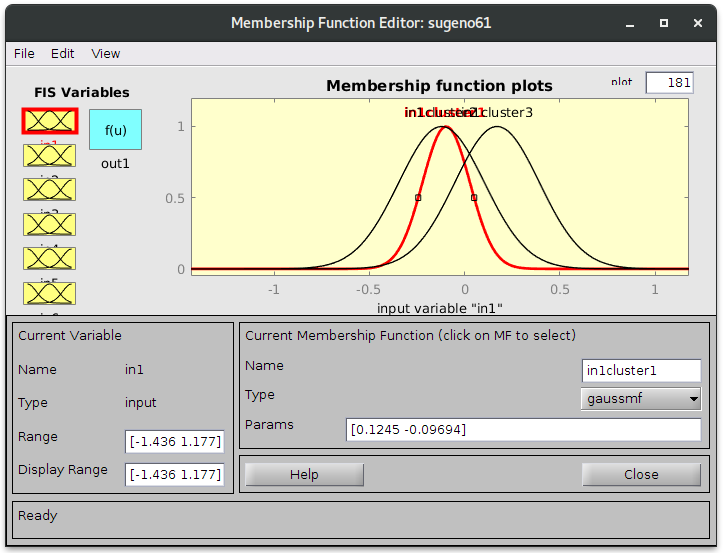
\includegraphics[height=1.2in]{images/fcm_hybrid_in1}
		\caption{Membership Functions for input $in1$}
	\end{subfigure}
	~ 
	\begin{subfigure}[t]{0.3\textwidth}
		\centering
		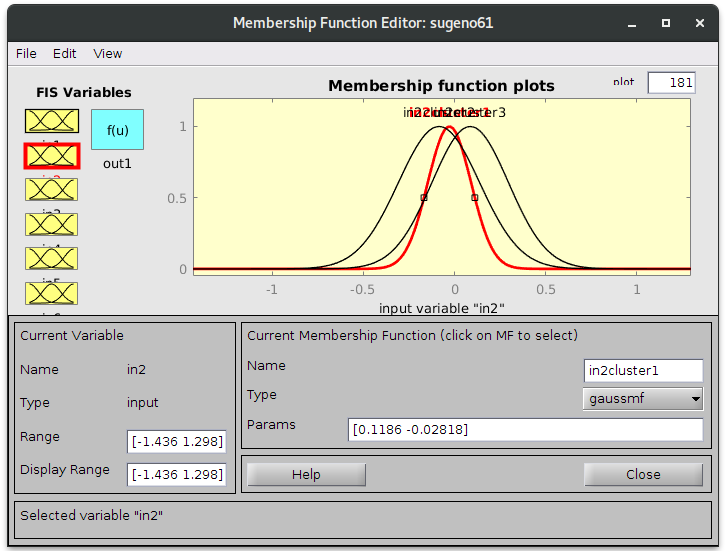
\includegraphics[height=1.2in]{images/fcm_hybrid_in2}
		\caption{Membership Functions for input $in2$}
	\end{subfigure}
	~
	\begin{subfigure}[t]{0.3\textwidth}
		\centering
		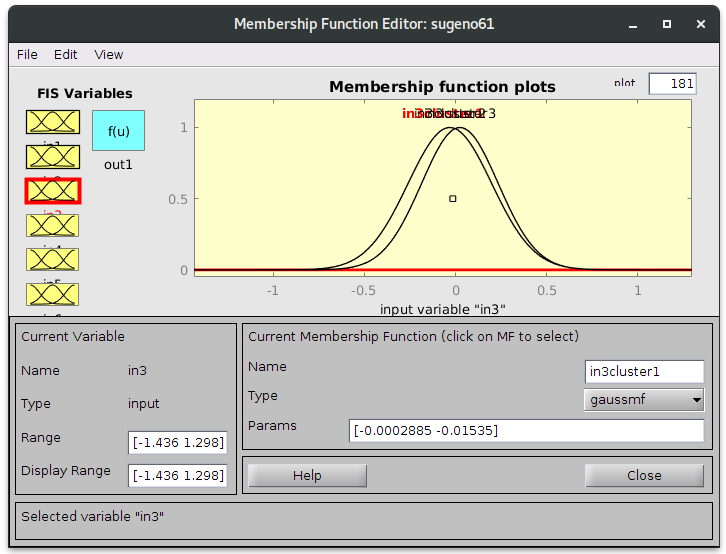
\includegraphics[height=1.2in]{images/fcm_hybrid_in3}
		\caption{Membership Functions for input $in3$}
	\end{subfigure}
	\\
	\begin{subfigure}[t]{0.3\textwidth}
		\centering
		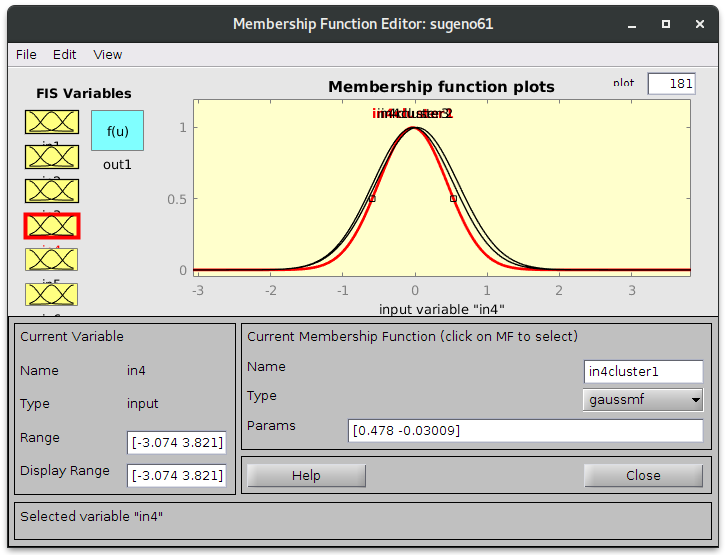
\includegraphics[height=1.2in]{images/fcm_hybrid_in4}
		\caption{Membership Functions for input $in4$}
	\end{subfigure}
	~ 
	\begin{subfigure}[t]{0.3\textwidth}
		\centering
		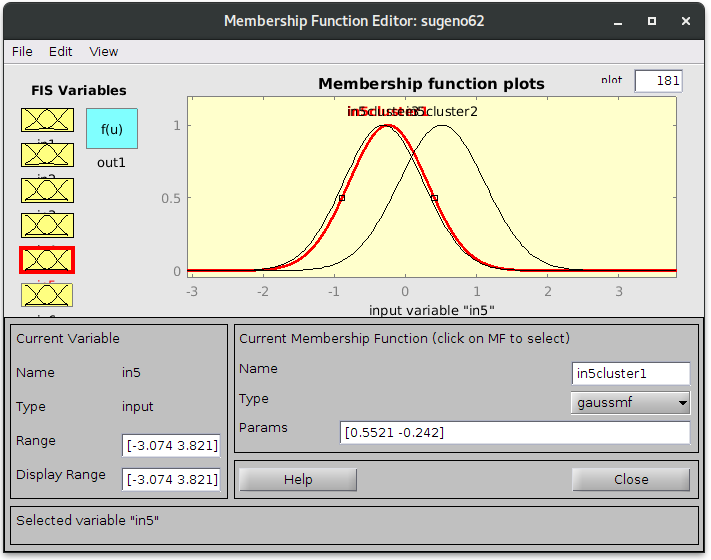
\includegraphics[height=1.2in]{images/fcm_hybrid_in5}
		\caption{Membership Functions for input $in5$}
	\end{subfigure}
	~
	\begin{subfigure}[t]{0.3\textwidth}
		\centering
		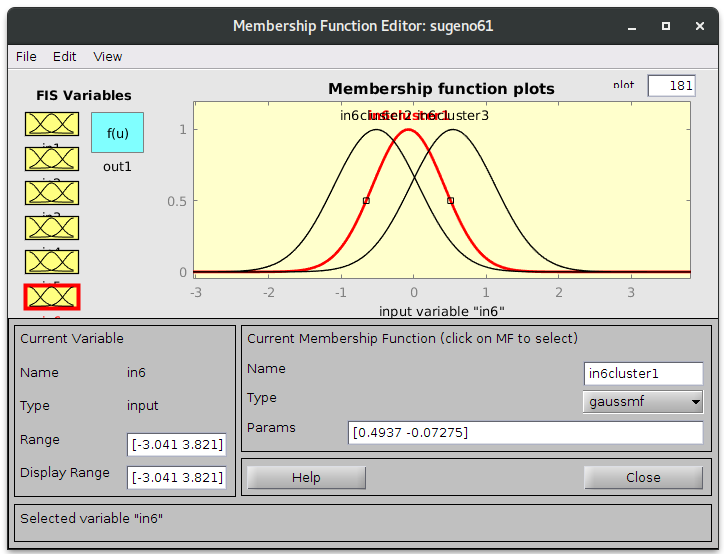
\includegraphics[height=1.2in]{images/fcm_hybrid_in6}
		\caption{Membership Functions for input $in6$}
	\end{subfigure}
	\caption{Input Membership Functions after Hybrid optimisation when the Fuzzy C-Means Clustering method was used in the rules initialisation.}
\end{figure}

Once the optimisation was complete, the performance of the final Neuro-Fuzzy Inference System was assessed using the test data. Table \ref{test_results} presents a summary of the results of the optimisation process. The error metric used to compute both the training and testing errors was the \emph{Root Mean Squared Error} (RMSE).

\begin{table}[ht]
	\begin{adjustwidth}{-1cm}{}
	\caption{Final results of the optimisation process.}
	\label{test_results}
	\begin{tabular}{|c|c|c|c|c|c|c|c|}
		\hline
		\textbf{\begin{tabular}[c]{@{}c@{}}Cluster\\ Technique\end{tabular}} & \textbf{\begin{tabular}[c]{@{}c@{}}Optimisation\\ Type\end{tabular}} & \textbf{\begin{tabular}[c]{@{}c@{}}Minimum\\ Training\\ Error\end{tabular}} & \textbf{\begin{tabular}[c]{@{}c@{}}Test\\ Error\end{tabular}} & \textbf{\begin{tabular}[c]{@{}c@{}}AND\\ Method\end{tabular}} & \textbf{\begin{tabular}[c]{@{}c@{}}OR\\ Method\end{tabular}} & \textbf{\begin{tabular}[c]{@{}c@{}}Number\\ Rules\end{tabular}} & \textbf{Order} \\ \hline
		Subtractive & Backpropagation & 9.1984e-17 & 0.0053 & prod & probor & 3 & 1 \\ \hline
		Subtractive & Hybrid & 1.5467e-06 & 8.9969e-04 & prod & probor & 3 & 1 \\ \hline
		Fuzzy C-Means & Backpropagation & 2.1481e-16 & 0.0044 & prod & probor & 3 & 1 \\ \hline
		Fuzzy C-Means & Hybrid & 1.5467e-06 & 1.5086e-06 & prod & probor & 3 & 1 \\ \hline
	\end{tabular}
	\end{adjustwidth}
\end{table}

\pagebreak

\section{Assessment Stage}
\label{fase_b}

Having developed and trained several NFSs to model the behaviour of the system presented in Section \ref{modelled_system} more diverse and intensive tests must be performed. With the goal of determining how close the developed NFSs were from the actual system a \emph{Simulink} model was developed and is presented in Figure \ref{assessment_simulink}.

\begin{figure}[ht]
	\centering
	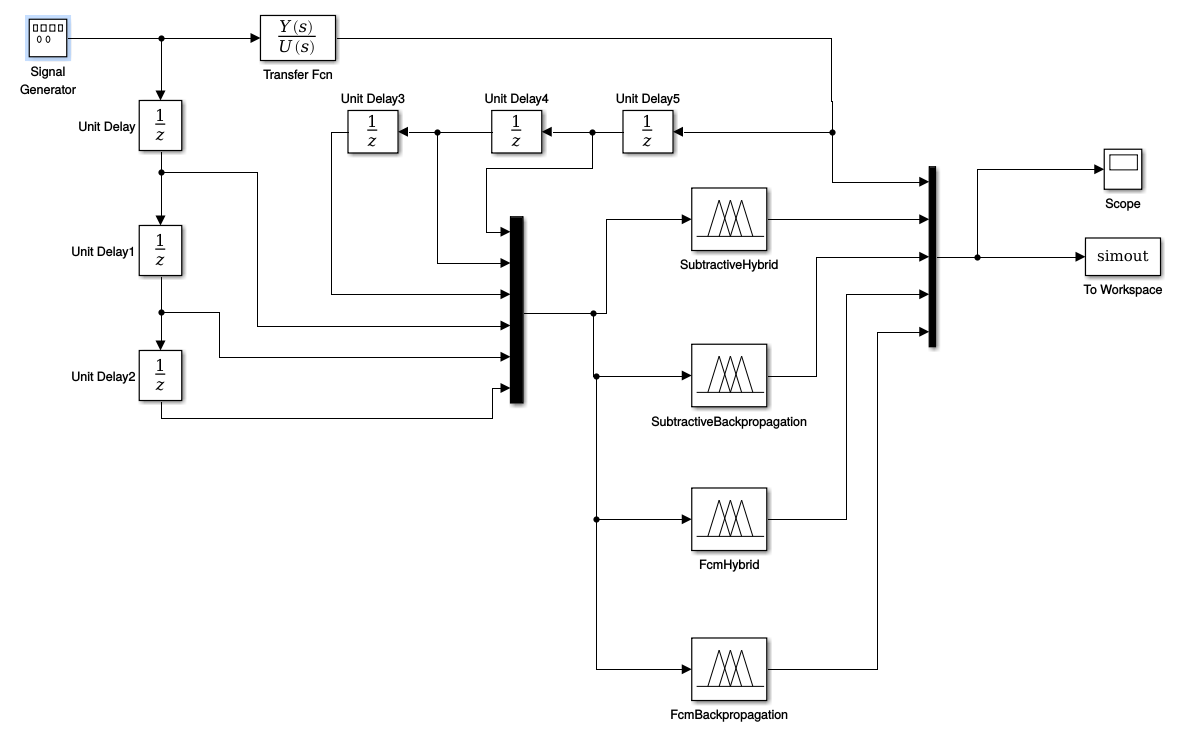
\includegraphics[scale=0.4]{images/assessment_simulink.png}
	\caption{Block diagram developed in Simulink to assess how close the developed NFSs were to the actual system to be modelled.}
	\label{assessment_simulink}
\end{figure}

In this exercise, a signal generator produces an input signal that is provided to the system being modelled (contained in the \emph{Transfer Func} block, described by the transfer function presented in Section \ref{modelled_system}) and to each one of the four NFSs developed in the previous stage. The five computed outputs were then inspected and plotted in the \emph{Scope} block.

Functions presented in the listing that follows were used in the \emph{Signal Generator} block to produce the input signals. Table \ref{results_table} presents the \emph{Root Mean Squared} (rmse) errors registered with each developed Neuro-Fuzzy System, for each input wave.

\begin{itemize}
	\item \emph{Sawtooth} wave, with an amplitude of $1$, units defined in \emph{Hertz} and a frequency set to the sampling interval whose computation was described in Section \ref{data_collection}.
		
	\item \emph{Sine} wave, with an amplitude of $1$, units defined in \emph{Hertz} and a frequency set to the sampling interval whose computation was described in Section \ref{data_collection}.
	
	\item \emph{Square} wave, with an amplitude of $1$, units defined in \emph{Hertz} and a frequency set to the sampling interval whose computation was described in Section \ref{data_collection}. 
\end{itemize}

\begin{table}[ht]
	\centering
	\caption{Root Mean Squared Errors of the different Neuro-Fuzzy Systems for the three input waves.}
	\label{results_table}
	\begin{tabular}{|c|c|c|c|}
		\hline
		\textbf{Wave Type} & \textbf{\begin{tabular}[c]{@{}c@{}}Cluster\\ Technique\end{tabular}} & \textbf{\begin{tabular}[c]{@{}c@{}}Optimisation\\ Type\end{tabular}} & \textbf{RMSE} \\ \hline
		Sawtooth & Subtractive & Hybrid & 3.0734e-04 \\ \hline
		Sawtooth & Subtractive & Backpropagation & 0.0051 \\ \hline
		Sawtooth & Fuzzy C-Means & Hybrid & 3.0734e-04 \\ \hline
		Sawtooth & Fuzzy C-Means & Backpropagation & 0.0031 \\ \hline
		
		Sine & Subtractive & Hybrid & 8.4137e-04 \\ \hline
		Sine & Subtractive & Backpropagation & 0.0056 \\ \hline
		Sine & Fuzzy C-Means & Hybrid & 5.7272e-05 \\ \hline
		Sine & Fuzzy C-Means & Backpropagation & 0.0041 \\ \hline
		
		Square & Subtractive & Hybrid & 3.4867e-04 \\ \hline
		Square & Subtractive & Backpropagation & 0.0059 \\ \hline
		Square & Fuzzy C-Means & Hybrid & 3.4867e-04 \\ \hline
		Square & Fuzzy C-Means & Backpropagation & 0.005 \\ \hline
	\end{tabular}
\end{table}

Analysing the results presented in Table \ref{results_table} considerably low $rmse$ error values were registered for the different wave types and trained NFSs. Such results suggest that the NFSs can accurately reproduce the dynamics of the system being modelled. Indeed, the plots presented in Figures \ref{results_sawtooth}, \ref{results_sine}, \ref{results_square} support these statements.

The smallest $rmse$ value was registered for the \emph{Sine} wave, using an hybrid optimisation method and initial cluster estimations with Fuzzy C-Means. Overall, hybrid optimisation lead to errors about one order of magnitude lower than performing optimisation with the backpropagation method.

\begin{figure}[H]
	\centering
	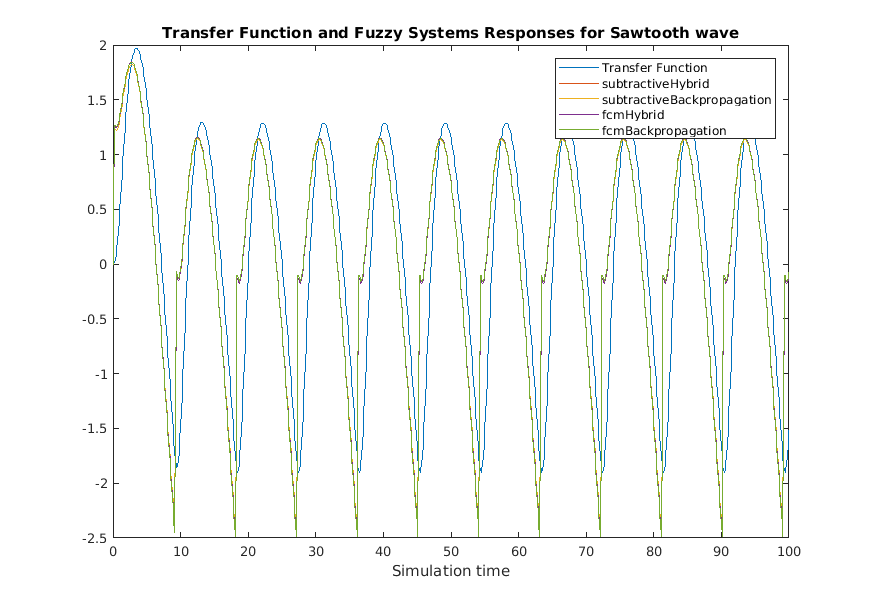
\includegraphics[scale=0.5]{images/assessment_sawtooth.png}
	\caption{Outputs of the system being modelled and the four NFSs developed when using the \emph{Sawtooth} wave to produce the inputs.}
	\label{results_sawtooth}
\end{figure}

\begin{figure}[H]
	\centering
	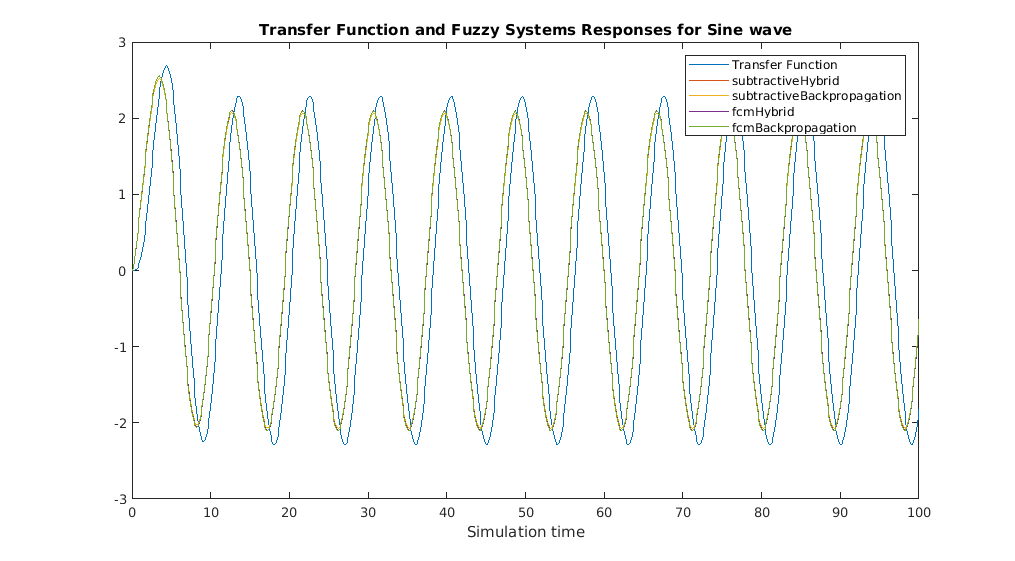
\includegraphics[scale=0.5]{images/assessment_sine.png}
	\caption{Outputs of the system being modelled and the four NFSs developed when using the \emph{Sine} wave to produce the inputs.}
	\label{results_sine}
\end{figure}

\begin{figure}[H]
	\centering
	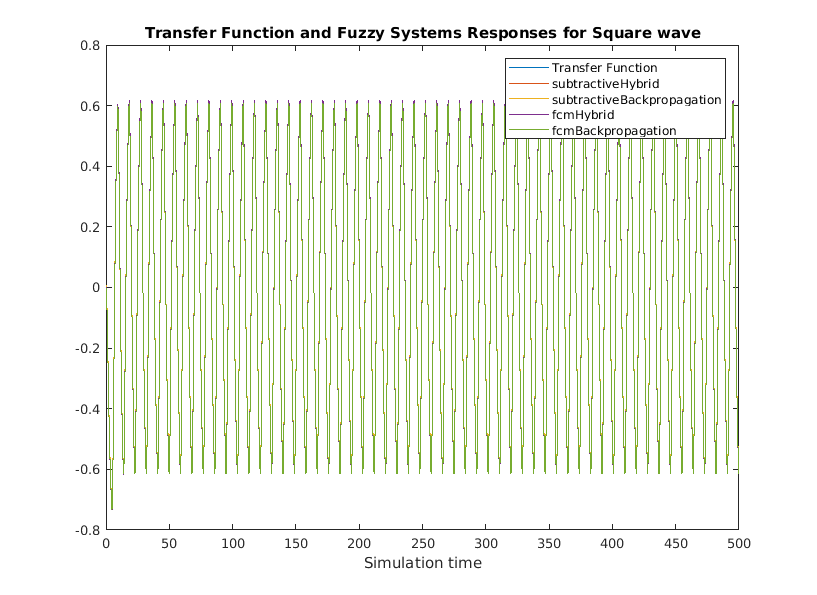
\includegraphics[scale=0.5]{images/assessment_square.png}
	\caption{Outputs of the system being modelled and the four NFSs developed when using the \emph{Square} wave to produce the inputs.}
	\label{results_square}
\end{figure}

\section{Conclusion}
\label{conclusion}

The current work focused on the task of modelling dynamic processes by means of Neuro-Fuzzy Systems. In the course of this work, such fuzzy logic controllers were projected and developed, based on the dynamics of a given system, described by a transfer function.

In an initial stage, a random input signal was provided to the \emph{"real"} system (that is, the one to be modelled) and its corresponding outputs were recorded. A dataset containing tuples with input signals and the respective system outputs was created to be used in the development of the Neuro-Fuzzy Systems. This development consisted in two main stages:

At first, estimates to the fuzzy rules that govern the operation of these systems were obtained by means of a clustering technique - two distinct clustering algorithms were considered: \emph{Subtractive} and \emph{Fuzzy C-Means} clustering.

In a second step, an optimisation of the initial rules estimates was performed using an \emph{ANFIS} structure. Two optimisation methods were also considered at this point - \emph{Backpropagation} and an \emph{Hybrid} optimisation method.

After the training, an initial performance assessment was conducted with part of the data initially collected. As presented in Table \ref{assessment_simulink}, the use of the \emph{Backpropagation} optimisation technique registered the lowest errors during training; however substantially worst results were registered during testing, suggesting a lack of generalisation for this optimisation method. On the other hand, the \emph{Hybrid} optimisation method was still capable of producing acceptable results in training which remained more stable during testing, suggesting a more general (and therefore desirable) model.

Based on the information mentioned, models developed using the \emph{Hybrid} optimisation method could be seen as good candidates to model the dynamics of the system in question. Indeed, further tests conducted with different input signals support such suggestions: using either a \emph{Sawtooth}, \emph{Square} or \emph{Sine} wave the use of \emph{Hybrid} optimisation always registered lower errors than when using \emph{Backpropagation}.

\end{document}